\chapter{Experiments}\label{chap:experiments}

Experiments often include benchmarks.
You need to describe you benchmarking setup: parameters of the machine used (architecture, memory, etc), parameters of the software used (OS version, libraries used and their version), the benchmark programs.
The programs need not be part of the thesis, but they should be described and available separately.

If you measure run times and evaluate your findings statistically, then there is great potential for errors.
Consult SIGPLAN's checklist for empirical evaluations \url{http://www.sigplan.org/Resources/EmpiricalEvaluation/} for advice. 

% \newsavebox{\mintedbox}

\begin{figure}[h]
\begin{centering}
    \subfloat[Some cool graphic]{
        {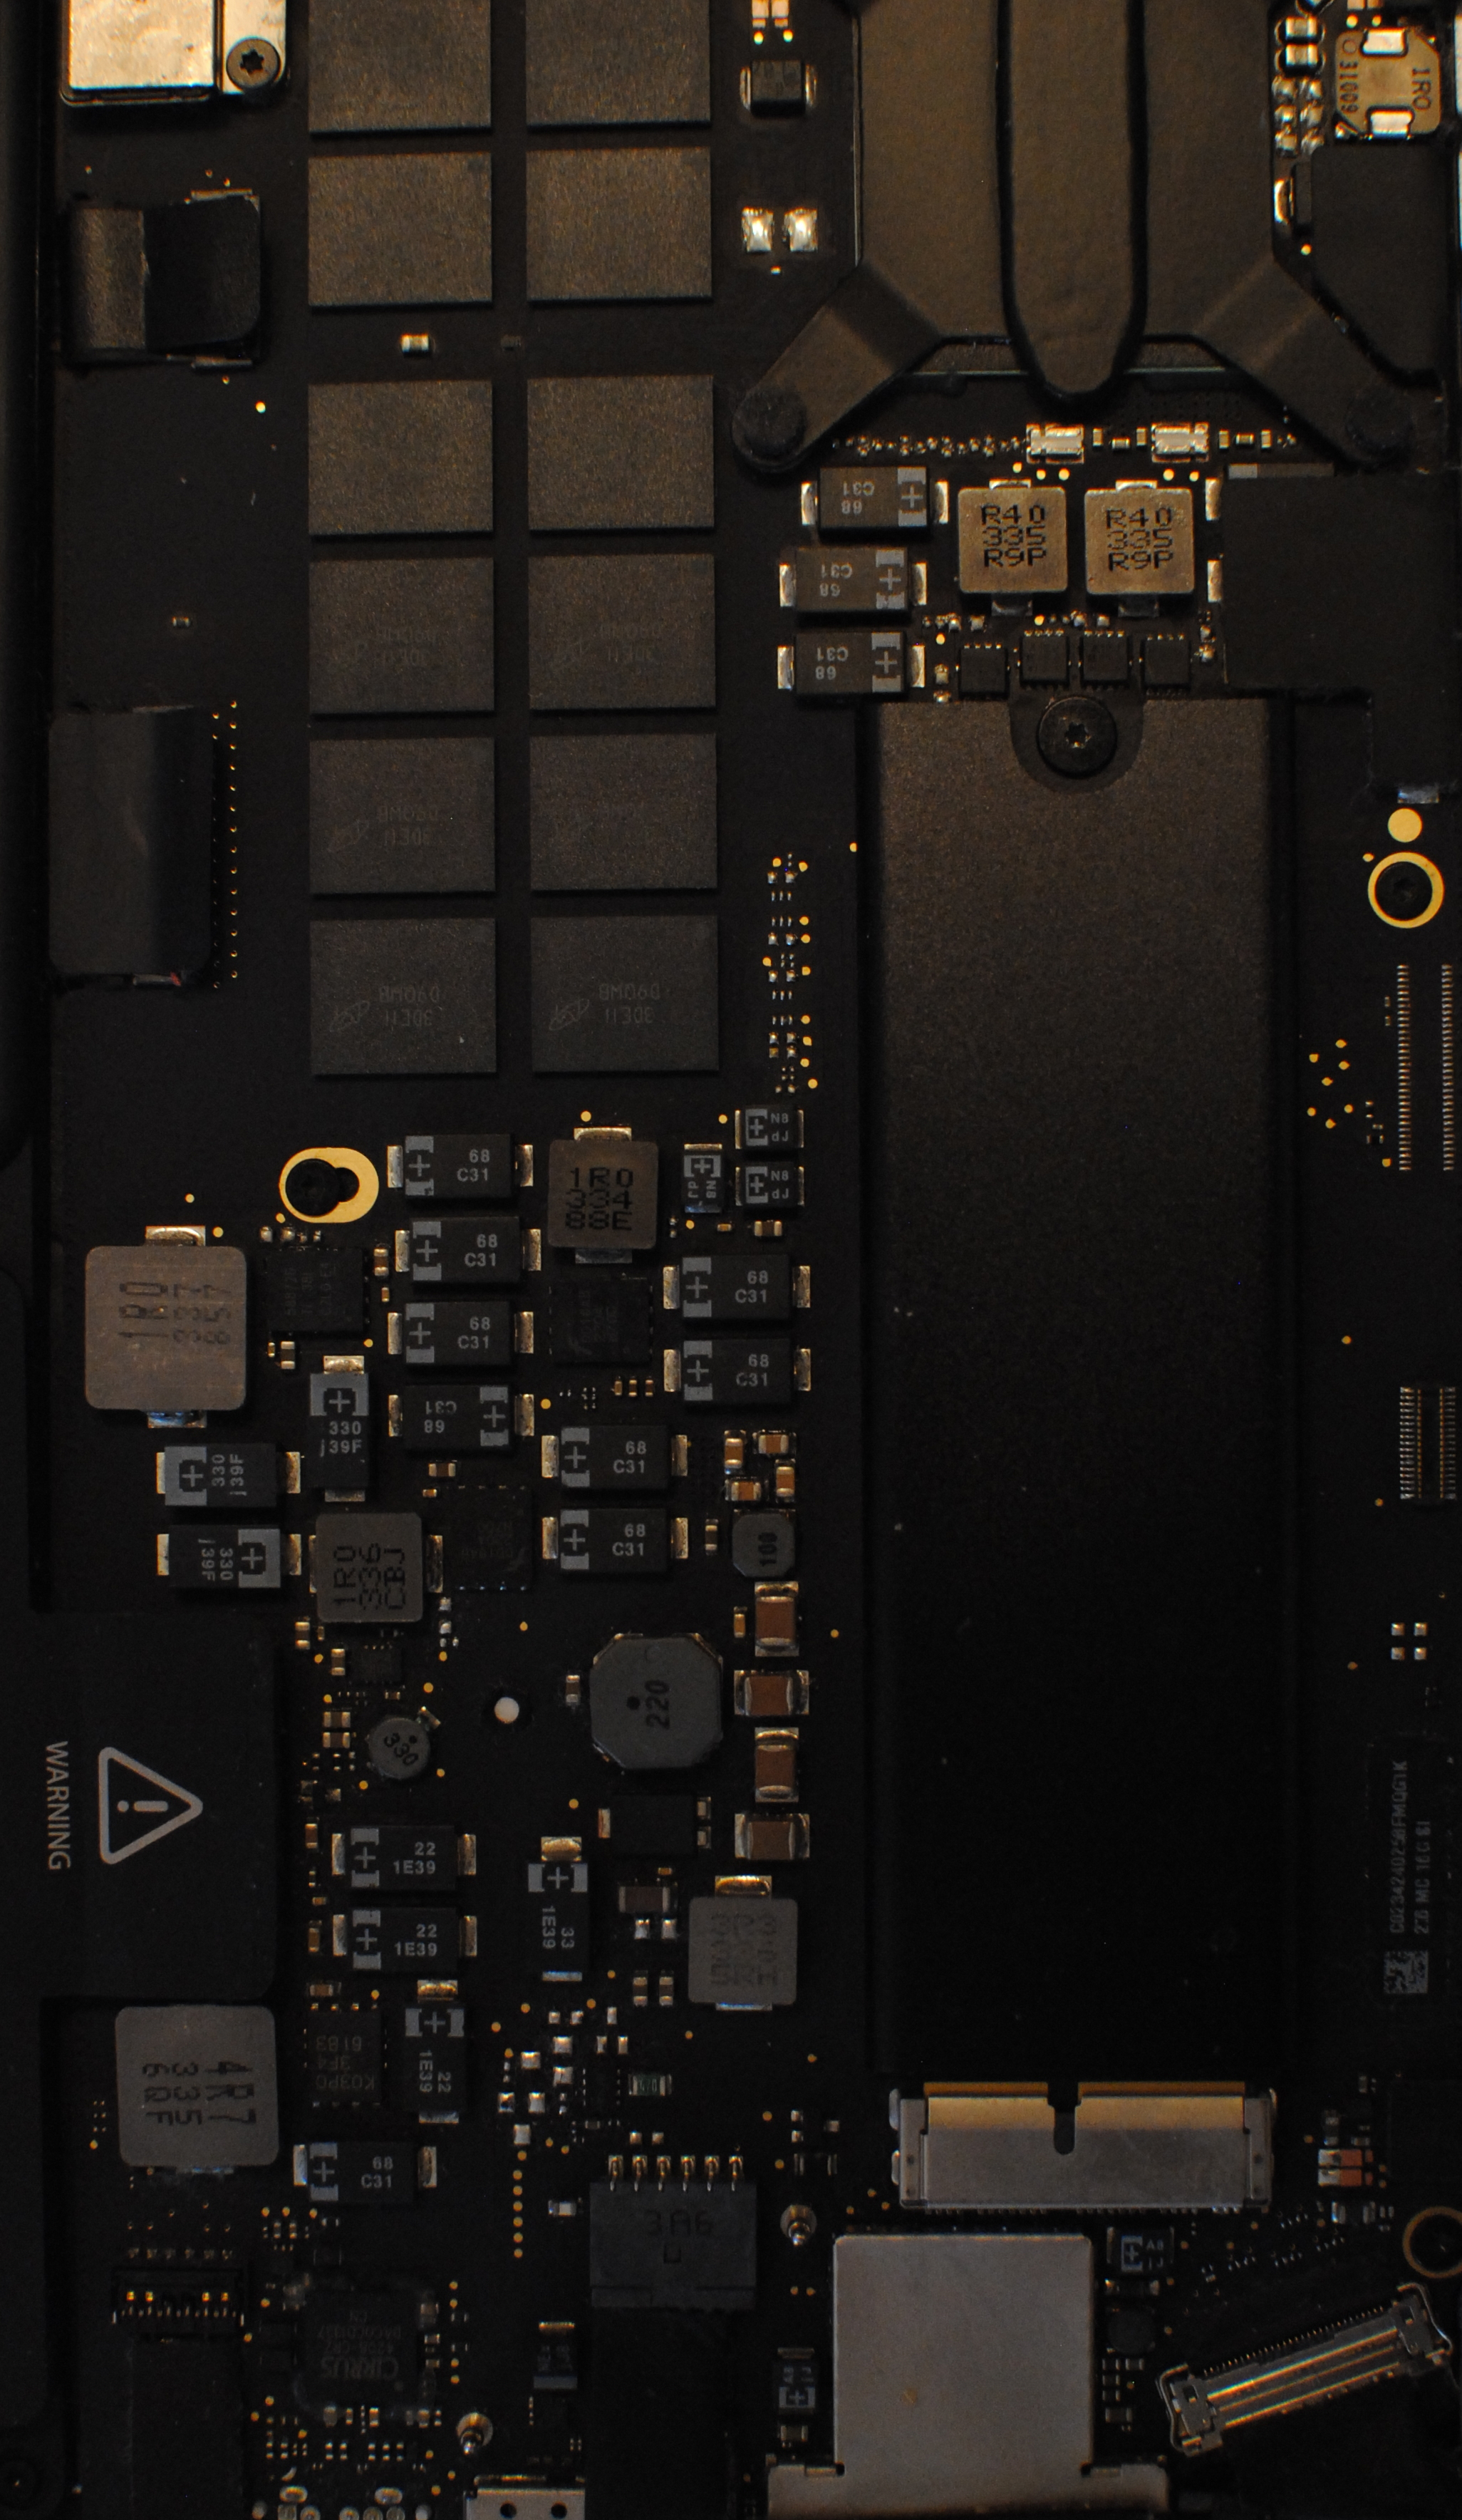
\includegraphics[scale=0.4]{figures/experiments/img.JPG}}
    }

    % \begin{lrbox}{\mintedbox}
    %     \begin{minipage}{\textwidth}
    %         \jscode{code/blacklisted-modules/A.js}
    %     \end{minipage}
    % \end{lrbox}
    % \subfloat[some code]{\usebox{\mintedbox}}

    \subfloat[Some cool related graphic]
    {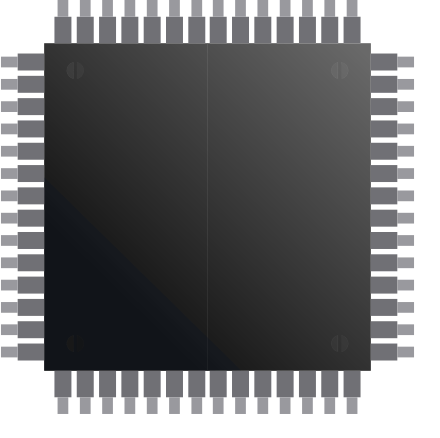
\includegraphics[scale=0.4]{figures/experiments/microcontroller.png}}
    \caption[Caption that appears in the figlist]{\textbf{Caption that appears under the fig} \lipsum[1-1]}
    \label{fig:pcaclasses}
\end{centering}
\end{figure}
\begin{table}[ht]
\begin{center}
    \begin{tabular}{|l|r|}
        \hline
        Type & Accuracy\\ \hline
        A    & 82.47 $\pm$ 3.21 \\
        B    & 78.47 $\pm$ 2.43 \\
        C    & 84.30 $\pm$ 2.35 \\
        D    & 86.81 $\pm$ 3.01 \\
        \hline
    \end{tabular}
    \end{center}

    \caption[Table caption]{\textbf{Table caption.} foo bar...\\}
    \label{tab:accuracy}
\end{table}

\section{Definitely Typed Modules}

\section{Code Examples Extraction}
\subsection{Repositories URL}
\subsection{Readme Files}
\subsection{Code Examples}

\section{Code Execution}

\section{Run-time Information Gathering}

\section{Declaration Files Generation}

\section{Evaluation}

\section{JS Operators Usage}